\documentclass{beamer}
\RequirePackage{preamble}
\usetheme{poisson}

\newcommand{\probability}{\mathbb{P}}

\title{De Poissonverdeling}
\subtitle[De Poissonverdeling]{Faculteit Militaire Wetenschappen}
\date[15-04-2024]{15 april 2024}
\author[Danny Blom]{dr. ir. Danny Blom}

\begin{document}
	
	\begin{frame}
		\maketitle 
	\end{frame}

	\begin{frame}		
		\resizebox{\linewidth}{!}{``Het leven is goed voor maar twee dingen:}
		\resizebox{\linewidth}{!}{wiskunde leren en wiskunde onderwijzen.''}
		
		\onslide<2>{
			\begin{figure}
				\includegraphics[scale=.1]{Figures/poisson.jpg}
				\caption*{Sim\'eon Poisson (1781 - 1840)}
			\end{figure}
			
		}
	\end{frame}


	\begin{frame}{Inhoud}
		\tableofcontents
	\end{frame}

	% Current section
	\AtBeginSection[ ]
	{
		\begin{frame}{Inhoud}
			\tableofcontents[currentsection]
		\end{frame}
	}

	%\section{Binomiale verdeling}
	
%	\begin{frame}{Binomiale verdeling}
%		Aantal ``successen'' in een eindig aantal onafhankelijke ``experimenten''. Wat is de kans dat:\\[2ex]
%		
%		\begin{itemize}
%			\item een luchtafweersysteem met succeskans $0.8$ acht van tien vijandelijke raketten onderschept?
%			%\item minstens een keer rood bij vijf spellen roulette?
%		\end{itemize}			
%	\end{frame}
%


	\section{De Poissonverdeling}
	
	\begin{frame}{De Poissonverdeling}
		
		\begin{itemize}
			\item tellen van ``events'' in een gegeven interval (tijd / ruimte)
			\item volgens gemiddelde regelmaat, onafhankelijk van elkaar
		\end{itemize}
	
		\vfill 
%				\begin{center}
%						\begin{tikzpicture}
%								% draw a horizontal line
%								\draw (0,0) -- (6,0);
%								
%								% draw vertical lines
%								\foreach \x in {0, 6}
%								\draw (\x cm,3pt) -- (\x cm,-3pt);
%								
%								% draw nodes to add events
%								\draw (0,0) node[below=3pt] {0} node[above=3pt] {};
%								\draw (6,0) node[below=3pt] {$t$} node[above=3pt] {};
%								
%								\foreach \x in {1.7, 2.6, 4.1, 4.3, 4.8}
%									\draw (\x, 0) node[draw, star, star points=5, star point ratio=2.25, blue, inner sep=.5pt, above=3pt] {};
%							\end{tikzpicture}
%					\end{center}
	
		Bijv. het aantal
		\begin{itemize}
			\item raketaanvallen in een oorlog op een dag
			\item storingen aan militair materieel in een jaar
			\item onontplofte explosieven op een km$^2$
		\end{itemize}
%		\vfill 
%		\begin{center}
%			\begin{tikzpicture}
%				% draw a horizontal line
%				\draw (0,0) -- (6,0);
%				
%				% draw vertical lines
%				\foreach \x in {0, 6}
%				\draw (\x cm,3pt) -- (\x cm,-3pt);
%				
%				% draw nodes to add events
%				\draw (0,0) node[below=3pt] {0} node[above=3pt] {};
%				\draw (6,0) node[below=3pt] {$t$} node[above=3pt] {};
%				
%				\foreach \x in {1.7, 2.6, 4.1, 4.3, 4.8}
%					\draw (\x, 0) node[draw, star, star points=5, star point ratio=2.25, blue, inner sep=.5pt, above=3pt] {};
%			\end{tikzpicture}
%		\end{center}
		
				
	\end{frame}
		
	\begin{frame}{De Poissonverdeling}
		
		Een toevalsvariabele $X$ is \textit{Poisson verdeeld} met parameter $\mu$ als voor alle $k = 0, 1, 2, \ldots$ geldt dat
		\[ \probability(X = k) = e^{-\lambda t} \cdot \frac{(\lambda t)^{k}}{k!} = e^{-\mu} \cdot \frac{\mu^{k}}{k!}, \]
		
		waarbij		
		
		\begin{itemize}
			\item $\mu = \lambda t$: verwacht aantal ``events'' (in een gegeven interval van $t$ meeteenheden),
			\item $e \approx 2.718...$: grondtal van de natuurlijke logaritme, en
			\item $k! = k \cdot (k-1) \cdot \ldots 2 \cdot 1$.
		\end{itemize}
	\vfill
	\textbf{Notatie}: $X \sim \textrm{Poisson}(\mu)$
	\end{frame}

	\begin{frame}{De Poissonverdeling: voorbeeld}
		Een team van de Explosieve Opruimingsdienst Defensie (EOD) werkt in een uitzendgebied aan het ruimen van zogenaamde ``improvised explosive devices'' (IED's). Het gemiddeld aantal IED's per hectare wordt geschat op 0.5.
		\vfill 
		Het team scant een gebied van 5 hectare, wat is de kans dat minstens 2 IED's worden gedetecteerd?
	\end{frame}
	
	\begin{frame}{De Poissonverdeling: voorbeeld}
		Uit het voorbeeld blijkt dat
		\begin{itemize}
			\item $\mu = \lambda t = 0.5 \cdot 5 = 2.5$ \hfill (5 hectares \`a 0.5 IED's per hectare)
			\item $k = 2$
		\end{itemize}
		\vfill
		Stel $X$ is de toevalsvariabele die het aantal gedetecteerde IED's telt.
		\vfill
		Er volgt dat $X \sim \textrm{Poisson}(\mu) = \textrm{Poisson}(2.5)$, dus
		\begin{align*}
			\probability(X  \ge 2) 	&= 1 - (\probability(X = 0) + \probability(X = 1)) \\
									&= 1 - (e^{-2.5} \cdot \frac{(2.5)^{0}}{0!} + e^{-2.5} \cdot \frac{(2.5)^{1}}{1!}) \\
									&\approx 0.713.
		\end{align*}
	\end{frame}
	
	\section{Connectie met andere kansverdelingen}
	
	\begin{frame}{Connectie met andere kansverdelingen}
		\begin{center}
			\textbf{Binomiale verdeling}
		\end{center}
	
		\begin{itemize}
			\item $n$: aantal experimenten
			\item $p$: succeskans
		\end{itemize}
	
		\vfill
	
		De toevalsvariabele $Y$ is \textit{binomiaal verdeeld} met parameters $n$ en $p$ als voor alle $k = 0, 1, \ldots, n$ geldt dat:
		\[\probability(Y = k) = \binom{n}{k} p^{k}(1-p)^{n-k} = \left(\frac{n!}{k!\cdot(n-k)!}\right) p^{k}(1-p)^{n-k} \]
		\textbf{Notatie:} $Y \sim $ Bin($n,p$)
	\end{frame}
	
	\begin{frame}{Connectie met andere kansverdelingen}
		
		De Poissonverdeling met parameter $\mu$ is een goede benadering voor de binomiale verdeling met parameters $n$ en $p = \frac{\mu}{n}$ als het aantal experimenten $n$ groot genoeg is:
		\vfill
		Voor alle $k = 0, 1, 2, \ldots$:
		\[ 
			 \text{Als } n \to \infty:\qquad \binom{n}{k} \cdot (\frac{\mu}{n})^{k} \cdot (1-\frac{\mu}{n})^{n-k} \approx e^{-\mu} \cdot \frac{\mu^{k}}{k!} 
		\]
				\vfill 
		\begin{center}
			Zie Python simulatie!
		\end{center}	
	\end{frame}

%	\begin{frame}{Connectie met andere kansverdelingen}
%		
%		Wiskundig gezien kun je bewijzen dat
%		\[ \lim\limits_{n \to \infty} \binom{n}{k} \cdot (\frac{\mu}{n})^{k} \cdot (1 - \frac{\mu}{n})^{n - k} = e^{-\mu}\cdot \frac{\mu^{k}}{k!} \]
%		
%	\end{frame}

	\begin{frame}{Connectie met andere kansverdelingen}
		Stel we bekijken een hectare van het conflictgebied en delen het op in veel kleine gebiedjes (bv. 1 meter bij 1 meter).
		\vfill
		\begin{itemize}
			\item Experiment: inspecteer een specifiek gebiedje
			\item ``Succes'': er ligt een IED in het gebiedje
		\end{itemize}
		\vfill		
		\begin{center}
			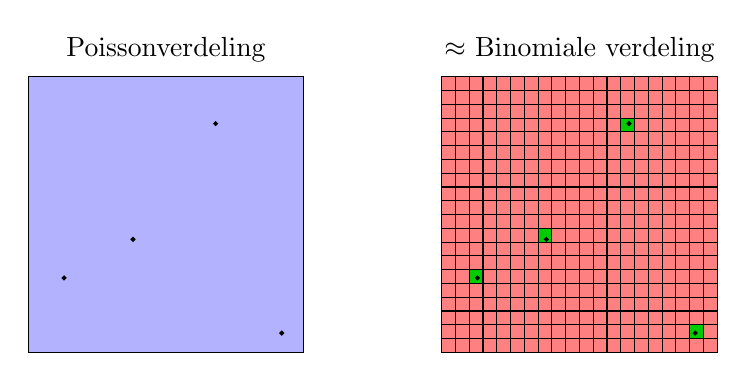
\begin{tikzpicture}[scale=0.35]
				\def\offset{15}
				
				\foreach \x in {0,.5,...,9.5}
					\foreach \y in {0,.5,...,9.5}
						\draw[fill=red!50] (\x+\offset, \y) -- (\x+0.5+\offset,\y) -- (\x+0.5+\offset, \y+0.5) -- (\x+\offset, \y+0.5) -- cycle;
				
				\draw[fill=green!80!black] (1+\offset, 2.5) -- (1.5+\offset, 2.5) -- (1.5+\offset, 3) -- (1+\offset, 3) -- cycle;
				\draw[fill=green!80!black] (3.5+\offset, 4) -- (4+\offset, 4) -- (4+\offset, 4.5) -- (3.5+\offset, 4.5) -- cycle;
				\draw[fill=green!80!black] (9+\offset, 0.5) -- (9.5+\offset, 0.5) -- (9.5+\offset, 1) -- (9+\offset, 1) -- cycle;
				\draw[fill=green!80!black] (6.5+\offset, 8) -- (7+\offset, 8) -- (7+\offset, 8.5) -- (6.5+\offset, 8.5) -- cycle;
				
				\filldraw (1.3+\offset, 2.7) circle (2pt);
				\filldraw (3.8+\offset, 4.1) circle (2pt);
				\filldraw (9.2+\offset, .7) circle (2pt);
				\filldraw (6.8+\offset, 8.3) circle (2pt);
				
				\node at (5+\offset, 11) {$\approx$ Binomiale verdeling};
				
				% Poissonverdeling
				\draw[fill=blue!30] (0,0) -- (10, 0) -- (10, 10) -- (0, 10) -- cycle;
				
				\filldraw (1.3, 2.7) circle (2pt);
				\filldraw (3.8, 4.1) circle (2pt);
				\filldraw (9.2, .7) circle (2pt);
				\filldraw (6.8, 8.3) circle (2pt);
				
				\node at (5, 11) {Poissonverdeling};
			\end{tikzpicture}
		\end{center}
		
	\end{frame}

	\begin{frame}{Connectie met andere kansverdelingen}
		\begin{center}
			\textbf{Exponenti\"ele verdeling}
		\end{center}
		\vfill
		
		\textbf{Tot nu toe}: ``events'' tellen in een gegeven interval. \\[2ex]
		
		\textbf{Nu}: afstand meten tot het volgende ``event''.
		\vfill
		\begin{itemize}
			\item Hoe lang tot de volgende storing aan militair materieel?
			\item Hoeveel hectare moet worden gescand tot de volgende IED wordt gedetecteerd?
		\end{itemize}
	\end{frame}

	\begin{frame}{Connectie met andere kansverdelingen}
				
		Deze twee beweringen zijn equivalent:
		
		\begin{enumerate}
			\item De afstand $T$ tot het volgende ``event'' is groter dan $t > 0$ meeteenheden
			\item In de komende $t$ meeteenheden worden geen ``events'' waargenomen.
		\end{enumerate}	
		\vfill
		In andere woorden:
		
		\[ \probability(T > t) = \probability(X = 0) = e^{-\lambda t} \cdot \frac{(\lambda t)^{0}}{0!} = e^{-\lambda t} \]
		
		$ \Rightarrow$ $T$ is \textit{exponentieel} verdeeld met parameter $\lambda$

	\end{frame}

	\begin{frame}{Connectie met andere kansverdelingen: voorbeeld}
		We bekijken opnieuw het voorbeeld van het EOD team. Naar schatting is het gemiddelde aantal IED's per hectare gelijk aan 0.5.
		\vfill 
		Wat is de kans dat het EOD team na het scannen van 3 hectare geen IED heeft gedetecteerd?
	\end{frame}

	\begin{frame}{Connectie met andere kansverdelingen: voorbeeld}
		Uit het voorbeeld blijkt dat
		\begin{itemize}
			\item $\lambda = 0.5$ (gemiddeld aantal IED's per hectare)
			\item $t = 3$ (aantal meeteenheden (hectares))
		\end{itemize}
		\vfill
		Er volgt dat:
		\[
			\probability(T  > 3) = \probability(X = 0) = e^{-\lambda t} = e^{-0.5 \cdot 3} \approx 0.223 
		\]
	\end{frame}

%	\section{Toepassingen in militaire besluitvorming}
%	
%	\begin{frame}{Andere toepassingen}
%		De Poissonverdeling kan ook in combinatie met machine learning gebruikt worden voor o.a. militaire besluitvorming.
%		\vfill
%		\begin{itemize}\setlength\itemsep{2em}
%			\item Voorspellingen in de toekomst
%			\begin{itemize}
%				\item Bijv. aantal gewonden in een conflict op een dag
%				\item Plannen van medische zorg en evacuatiehandelingen
%			\end{itemize}
%			\item Classificatie van verdacht cyberverkeer
%			\begin{itemize}
%				\item Hoeveelheid verstuurde data in een minuut
%				\item Voorkomen van DDoS-aanvallen (uitzonderlijk hoge waardes)
%			\end{itemize}
%		\end{itemize}
%	\end{frame}

	\section{Samenvatting}
	
	\begin{frame}{Samenvatting}
		\begin{center}
			\begin{itemize}
				\item \textbf{Poisson}: ``events'' tellen in een interval (tijd / ruimte)
				\item Binomiale verdeling met grote $n$ en kleine $p$
				\item Exponenti\"ele verdeling: afstand tot het volgende ``event''
				\item Handige statistische tool voor o.a. militaire besluitvorming
			\end{itemize}\pause
		\end{center}
		\vfill
		\Huge\centering Vragen?\pause
		\vfill
		\Huge\centering Dank jullie wel!	
	\end{frame}
\end{document}
